\documentclass[11pt]{article}

\usepackage[margin=1in]{geometry}
\usepackage{amsmath}
\usepackage{microtype}
\usepackage{booktabs}
\usepackage{longtable}
\usepackage{array}
\usepackage{enumitem}
\usepackage{caption}
\usepackage{graphicx}
\usepackage[numbers,sort&compress]{natbib}
\usepackage[hidelinks]{hyperref}
\setlength{\emergencystretch}{2em}
\captionsetup[table]{width=0.96\linewidth,justification=raggedright,singlelinecheck=false}

%% Generated by scripts/paired_scope_table.py -- do not edit.
\newcommand{\pairedModelCount}{14}
\newcommand{\pairedDropMeanReward}{0.087}
\newcommand{\pairedDropPassAtK}{0.029}
\newcommand{\pairedDropRatio}{3.0}


\title{BioTerm-Bench v1: A Harbor-Compatible Benchmark for Tracking\\Open-Model Progress on Terminal Bioinformatics Tasks}
\author{
Petr Simecek\thanks{Corresponding author: \texttt{simecek@mail.muni.cz}} \quad Vojtech Bystry\\[0.5em]
\normalsize Central European Institute of Technology (CEITEC), Masaryk University, Czechia
}
\date{August 13, 2026}

\begin{document}
\sloppy
\maketitle

\begin{abstract}
Can a language model do your routine command-line bioinformatics unaided?
For a surprising share of everyday work, the answer is already yes---and it is small, openly licensed models running on ordinary hardware that get there, not only frontier systems behind an API.
BioTerm-Bench measures this directly: 32 self-contained tasks in which an agent is given real files, a container with the usual tools, and an exact specification of the output it must produce, and is graded by comparing that output against a known-correct answer.
Evaluation is fully deterministic: no model judges another model's output, and grading reduces to comparison against a stored correct artifact.
Examining agents on a basic set of 25 tasks, we found the benchmark already saturated---the strongest small open models solve essentially everything, one reaching 0.969 mean reward and answering all 25 correctly on its first attempt---so we added a frozen extension of harder multi-stage workflows.
Across 14 models on two independently reported infrastructures, that extension separates models over a wide range (mean reward 0.433--0.875) while remaining unsaturated.
Two findings matter most for practice.
First, difficulty lives in \emph{reliability}, not in what a model can eventually do.
What matters for unattended analysis is that an agent succeeds almost every time, so alongside mean reward we report the fraction of tasks a model solves on \emph{all four} attempts---a far more demanding criterion than solving a task at least once, and the one that corresponds to trusting a result without re-running it.
Allowing four attempts and keeping the best hides most of the gap: on the extension all five models of one cohort solve every task under best-of-four and are therefore indistinguishable, yet under the all-four criterion they span two to seven tasks out of seven.
Second, when these agents fail, the single most common outcome is not a crash or an unreadable file but a well-formed artifact containing wrong numbers (43.6\% of 319 scored failures)---the failure mode least likely to be noticed downstream.
The tasks, containers, graders, and analysis code are released freely so that a single laboratory can rerun the whole evaluation locally, including on infrastructure where sensitive genomic data must never leave the institution.
\end{abstract}

\section{Introduction}

A great deal of bioinformatics is not discovery.
It is converting a GTF to a BED, checking that a BAM is coordinate-sorted, pulling allele frequencies out of a VCF, normalising counts to TPM---work that is precisely specified, tedious, and easy to get subtly wrong.
This is exactly the shape of work where large language model (LLM) agents have started to be genuinely helpful, and the practical question for a laboratory is which parts can be delegated and how often the result will be right.

Answering that question requires a benchmark with three properties that existing ones do not combine.
It must run the tools rather than describe them, because an agent that writes a plausible \texttt{bcftools} invocation has not produced a filtered VCF.
It must grade deterministically, because an LLM judge drifts between versions and cannot be audited by the person relying on it.
And it should run on a laptop or an institutional node, so that the evaluation is cheap to repeat and so that it remains available for the subset of work where data cannot leave the institution.

There are large parts of bioinformatics without such constraints.
Model-organism genetics, public reference data, and most method development can be sent anywhere, and for that work the case for local execution is ordinary rather than regulatory: cost, reproducibility, and not depending on an API that may be retired.
But a substantial part of the field does carry the constraint, and it is the part where mistakes are most expensive: human genomic data under controlled access generally cannot be sent to unauthorised public generative-AI services \citep{nih2025genomicai}.
For that work the realistic deployment is federated, with the agent running where the data already sits and orchestrating ordinary command-line tools on a node that exports nothing.
Designing for the stricter case costs the easier one nothing, so three choices follow.
Tasks are sized for smaller, locally runnable open models rather than only frontier APIs.
Grading is fully deterministic, so a node can verify agent output automatically without calling out to anything.
Reference data, tools, and graders are containerised, so the same evaluation reproduces on a laptop, a cluster node, or a partner institution's hardware.

Running that evaluation across 14 models produced a result we did not expect to state so bluntly: the 25-task core is largely solved.
Two models answer all 25 tasks correctly on every one of four attempts.
That is genuinely good news for practitioners---routine terminal work is now largely automatable by models a laboratory can host itself---and it is bad news for the benchmark, because a scoreboard where several entrants are perfect no longer ranks anything.
So we did what benchmark maintainers must eventually do and built a harder pack, selecting eight multi-stage tasks before running any evaluation model, one of which we later retired, in the spirit of successively harder ARC-AGI generations.

What that harder pack revealed is the part most relevant to anyone deciding whether to hand work to an agent.
The extension is not harder because models cannot eventually solve it; given four attempts, several solve nearly all of it.
It is harder because models solve it \emph{unreliably}, and reliability is what a single-shot user actually consumes.
We therefore report mean reward---the fraction of individual attempts that come out right---as the primary number throughout, and treat best-of-four as a diagnostic rather than a score.

\section{Related work, and the principles BioTerm-Bench stands on}

BioTerm-Bench follows the executable-task tradition established by Terminal-Bench, which evaluates agents on hard, realistic tasks in genuine command-line environments and grades them with comprehensive tests \citep{merrill2026terminalbench}.
We adopt that model directly: our tasks run under Harbor, the Terminal-Bench harness, so the suite is a domain-specific pack within an existing ecosystem rather than a new framework \citep{harbor2026}.
The contribution is the domain instantiation---bioinformatics file formats, tools, and pipelines---together with three properties that, to our knowledge, no existing biological benchmark combines.

\paragraph{Executable artifacts rather than code.}
BioCoder evaluates function-level bioinformatics code generation against unit tests \citep{tang2024biocoder}, and ScienceAgentBench asks for a self-contained program derived from a published analysis \citep{chen2025scienceagentbench}.
Both are careful tests of code generation.
BioTerm-Bench instead supplies input files and a tool stack and holds the agent responsible for the final artifact, which shifts the difficulty toward format edge cases, coordinate conventions, and header requirements---the errors that dominate practical work.

\paragraph{Deterministic grading.}
BixBench evaluates open-ended exploration of biological datasets \citep{mitchener2025bixbench}, BLADE compares an agent's analysis against expert-validated alternatives \citep{gu2024blade}, and BioAgent Bench grades end-to-end workflow outputs using an LLM judge \citep{fa2026bioagentbench}.
Model-based grading is appropriate for open-ended questions, where no single output is uniquely correct.
It also introduces a dependency that changes as the judge model changes.
Because every BioTerm-Bench task states its output contract precisely, grading reduces to comparison against a stored answer, which keeps scores comparable across time and auditable by the user.

\paragraph{Local execution.}
BioAgent Bench shares our motivation regarding sensitive data but is built around cloud infrastructure \citep{fa2026bioagentbench}.
Closest in deployment assumptions is a recent evaluation of open-weight agents on longitudinal cohort-data preparation, motivated by governance rules that prohibit cloud transmission \citep{nixon2026nocloud}; that work targets data cleaning rather than bioinformatics file and tool pipelines.
Our fixtures are small enough to run on a laptop, and reference data, tools, and graders are containerised.

Benchmarks addressing scientific judgement are complementary.
BioDSA-1K evaluates hypothesis validation across biomedical studies \citep{wang2025biodsa}, and GeneBench-Pro targets multistage analyses in which a plausible wrong analytical choice changes the conclusion \citep{li2026genebenchpro}.
Those benchmarks ask whether an agent reaches a defensible scientific conclusion.
BioTerm-Bench addresses the prior question of whether it can reliably produce a specified artifact, which is a weaker requirement but one that can be verified exactly.

\section{Benchmark and analysis protocol}

The suite contains 32 deterministic tasks in two parts: a 25-task core and a seven-task extension of harder multi-stage workflows added once the core began to saturate.
Every task supplies a bounded local dataset, a container with the usual bioinformatics stack, an instruction that fixes the output contract exactly, and a verifier that returns a binary reward.
Table~\ref{tab:categories} summarises what the tasks cover.

\begin{table}[tbp]
\centering
\small
\caption{What the suite covers. Core tasks are single operations on one or two files; extension tasks chain several stages, so an error early in the chain is not recoverable later.}
\label{tab:categories}
\begin{tabular}{llp{7.6cm}}
\toprule
Category & Tasks & Examples \\
\midrule
alignment & 7 & BAM depth histograms, duplicate marking, soft-clipping statistics, SAM/CRAM round-trips, splice-junction support \\
variant & 7 & allele frequencies, normalisation, splitting by type, trio Mendelian checks, diploid consensus, compound heterozygotes, multi-sample QC \\
metadata & 6 & GTF to BED, longest ORF, header renaming, six-frame codon counts, longest-transcript CDS \\
quality control & 6 & per-base quality, FastQC-style summaries, paired-read adapter and orphan handling, contamination mixtures \\
search & 5 & best BLAST hit, MAFFT alignment identity, $k$-mer Jaccard matrices, reciprocal-best-hit ortholog clusters \\
RNA-seq & 4 & TPM normalisation, biotype summaries, featureCounts-style matrices, differential-expression contrasts \\
\bottomrule
\end{tabular}
\end{table}

Two terms recur.
An \emph{agent} is the loop wrapped around a language model that lets it act rather than answer: it issues a shell command, reads what came back, decides the next command, and stops when it judges the task done.
A \emph{harness} is the software that runs that loop reproducibly---starting the container, enforcing timeouts, capturing the transcript, and invoking the grader.
We use Harbor as the harness and hold the Terminus-2 agent fixed across all model comparisons, so that differences in score reflect the model rather than the scaffolding \citep{harbor2026}.
Throughout, a \emph{trial} is one attempt by one model at one task, \emph{reward} is the binary verifier outcome of a trial, and $k$ is the number of attempts per task.
pass@1 is the fraction of tasks solved on the first scheduled attempt, and pass@$k$ the fraction solved on at least one of $k$ attempts.

A worked example of one task---its fixture, exact output contract, and grader---is given in Appendix~\ref{app:example}.

Fixtures are reproducible by construction rather than novel by construction.
Each is rebuilt by a script in the repository, either as a deterministic reduction of reference data shipped inside the image or from a fixed random seed, and the regeneration commands are recorded so a reviewer can reconstruct any fixture.
This supports reproduction and auditing, but it is not a contamination guarantee: inputs derived from public reference annotation could in principle be memorized, even though the required output contract is task-specific and the graders demand exact artifacts.

The repeated-run setting used in the main analysis is the clean OpenRouter $k=4$ sweep already stored in this repository: 25 tasks, 4 attempts per task, and therefore 100 trials per model.
We analyze all job directories matching \texttt{jobs/full25-k4-open-*}.

The main complication is operational filtering.
We do not merge protocol failures with ordinary benchmark failures.
Instead, each completed job is classified from the raw trial artefacts using three rules:

\begin{enumerate}[leftmargin=1.5em]
\item unfinished jobs are excluded;
\item a trial is an error if it has non-null \texttt{exception\_info} or lacks a scored verifier reward;
\item jobs with error rate above 20\% are excluded as protocol failures.
\end{enumerate}

The 20\% threshold is a convention rather than a tuned optimum, and it is not load-bearing: eight of the nine jobs excluded on this rule have error rates of 0.97 or above and the ninth is 0.60, so any cut between roughly 0.25 and 0.55 gives the same partition.
It also handles a subtle but important case visible in the stored artefacts: Harbor can record a verifier reward of 0.0 on a trial that also has an explicit timeout exception, and such a trial should still count as an operational error rather than as a valid scientific zero.

\paragraph{Metrics.}
Our headline number is \emph{mean reward}: the fraction of all scored attempts that produced a correct artifact.
It answers the question a practitioner faces---if I hand this model one task, how often is the result right?---and uses every attempt rather than collapsing four into a binary.

Because unattended analysis needs an agent that succeeds \emph{almost every time}, we also report the \emph{all-attempts} rate: the fraction of tasks a model solved on all four attempts.
This is deliberately demanding, and it is the criterion that corresponds to trusting an output without re-running it.
We report pass@1 as a secondary single-shot view, and pass@$k$ only as a contrast, because counting a task as solved when any of four attempts succeeds presupposes an oracle that identifies which attempt was right---the benchmark has one, a working scientist usually does not.
Pass proportions carry exact Clopper--Pearson intervals over explicit scored denominators; mean-reward intervals are bootstrapped over task-level means.
Cost and wall-clock are retained as operational diagnostics, not speed claims, because the runs used shared hosted services.

\paragraph{Operational filtering.}
Provider failures are not benchmark failures.
Each completed job is classified from raw trial artefacts: unfinished jobs are excluded, a trial is an error if it carries an exception or lacks a scored verifier reward, and jobs whose error rate exceeds 20\% are excluded as protocol failures.
The threshold is a convention rather than a tuned optimum and is not load-bearing here---eight of the nine jobs it excludes have error rates above 0.97 and the ninth is 0.60.
The rule also catches a subtle case: Harbor can record a reward of 0.0 on a trial that also timed out, which is an operational error rather than a scientific zero.

\section{Results}
\label{sec:results}

\subsection*{The original 25 tasks are saturated}

Table~\ref{tab:headline} reports the clean repeated OpenRouter cohort on the core: 23 jobs, of which 8 are usable and 15 are excluded as unfinished or operationally broken.
The top of the table is saturated.
Gemma~4~26B~A4B reaches 0.969 mean reward and solves all 25 tasks on its first attempt, with Qwen~3.5~9B at 0.878 and Gemma~4~31B at 0.920.
With only 25 task units the exact 95\% interval for a perfect score is still 0.863--1.000, so adjacent rows overlap heavily and the table stratifies models into bands rather than ranking them; a small-model panel whose leader misses three of 98 scored attempts is itself the saturation signal.
Category rates are flat (pooled pass@4 of 0.75 for alignment, quality control, RNA-seq and search, 0.69 for metadata, 0.68 for variant), so the core behaves as a competence floor rather than a separating leaderboard.

\begin{table}[t]
\centering
\small
\caption{Included OpenRouter $k=4$ runs on the 25-task core, ordered by mean reward. Pass denominators are explicit scored-task counts.}
\label{tab:headline}
\begin{tabular}{lrrrrrr}
\toprule
Model & mean reward & pass@1 & all-scored & mixed & pass@4 & Cost (USD) \\
\midrule
Gemma 4 26B A4B & 0.969 & 25/25 & 22/25 & 3/25 & 25/25 & 0.29 \\
Qwen 3.5 9B & 0.878 & 24/25 & 18/25 & 7/25 & 25/25 & 1.37 \\
Gemma 4 31B & 0.920 & 22/25 & 22/25 & 2/25 & 24/25 & 0.20 \\
GPT-OSS 20B & 0.520 & 11/25 & 6/25 & 17/25 & 23/25 & 0.08 \\
Mistral Small 3.2 24B & 0.380 & 8/22 & 5/25 & 11/25 & 16/25 & 2.22 \\
Qwen 3 30B A3B & 0.283 & 7/24 & 2/25 & 11/25 & 13/25 & 0.92 \\
Qwen 3 14B & 0.381 & 9/20 & 3/25 & 9/25 & 12/25 & 1.15 \\
Qwen 3 8B & 0.131 & 3/20 & 1/25 & 5/25 & 6/25 & 0.70 \\
\bottomrule
\end{tabular}

\end{table}

Repeated attempts still carry information even here: GPT-OSS~20B scores 0.520 mean reward while solving 11 of 25 tasks on the first attempt and 23 of 25 within four, which is exactly the gap a best-of-$n$ report would hide.
Operational failures are common enough to matter---the excluded set includes several 100/100-error jobs, and a billed Mistral~Small~3.1~24B run is not scored because all 100 trials carry \texttt{AgentTimeoutError}.

\subsection*{A harder extension, and whether it discriminates}

We therefore froze a harder pack of eight multi-stage tasks, selected on three development models before any evaluation model ran, requiring each candidate to show at least one pass and one failure at a pooled development pass rate between 10\% and 80\%.
The procedure is transparent but circular by construction---tasks were kept because they separated three particular models---so the evaluation panel is a held-out test of the selection rule itself.
Appendix~\ref{app:selection} holds the per-task receipt.

Two cohorts answer the question, run under the identical protocol and reported separately because provider and model set are confounded across them: nine models on e-INFRA (Table~\ref{tab:hard8-einfra}) and five on OpenRouter (Table~\ref{tab:hard8-openrouter}).

\begin{table}[t]
\centering
\small
\caption{Extension, e-INFRA cohort (August 13--14, 2026), all nine models scored. \texttt{kimi-k3} is scored from a re-run after a provider outage invalidated its first attempt; both receipts are retained.}
\label{tab:hard8-einfra}
\begin{tabular}{lrrrrr}
\toprule
Model & mean reward & pass@1 & all-scored & mixed & pass@4 \\
\midrule
Deepseek V4 Flash Thinking & 1.000 & 7/7 & 7/7 & 0/7 & 7/7 \\
Deepseek V4 Flash & 0.923 & 6/7 & 5/7 & 2/7 & 7/7 \\
Glm 5.2 & 0.929 & 6/7 & 6/7 & 1/7 & 7/7 \\
Kimi K3 & 0.964 & 6/7 & 6/7 & 1/7 & 7/7 \\
Mistral Medium 3.5 & 0.926 & 6/7 & 6/7 & 1/7 & 7/7 \\
Qwen3.5 Int4 & 0.964 & 6/7 & 6/7 & 1/7 & 7/7 \\
Gemma4 & 0.786 & 5/7 & 5/7 & 2/7 & 7/7 \\
Qwen3.5 122B & 0.679 & 5/7 & 2/7 & 4/7 & 6/7 \\
Gpt Oss 120B & 0.423 & 3/6 & 1/7 & 3/7 & 4/7 \\
\bottomrule
\end{tabular}

\end{table}

\begin{table}[t]
\centering
\small
\caption{Extension, OpenRouter cohort. Cost is billed provider cost, reported only because this provider bills per token.}
\label{tab:hard8-openrouter}
\begin{tabular}{lrrrrrr}
\toprule
Model & mean reward & pass@1 & all-scored & mixed & pass@4 & Cost (USD) \\
\midrule
GPT-5.6 Luna & 1.000 & 7/7 & 7/7 & 0/7 & 7/7 & 0.13 \\
Inkling Small & 1.000 & 7/7 & 7/7 & 0/7 & 7/7 & 0.59 \\
Muse Glimmer 30B & 1.000 & 7/7 & 7/7 & 0/7 & 7/7 & 1.64 \\
Qwen 3.6 35B A3B & 0.821 & 6/7 & 4/7 & 3/7 & 7/7 & 0.72 \\
Nemotron 3.5 Lightning & 0.571 & 4/7 & 2/7 & 5/7 & 7/7 & 0.36 \\
\bottomrule
\end{tabular}

\end{table}

The answer is a qualified yes.
Across the fourteen scored models mean reward runs from 0.423 to 1.000 on e-INFRA and from 0.571 to 1.000 on OpenRouter, so the extension separates capability over a wide range.
It nonetheless saturates at the top, and one retired task is the reason.

\paragraph{One task was retired, and it cost the subset its ceiling.}
\texttt{bam-splice-junction-support} was solved by 2 of the 14 scored models, with a per-task mean reward of 0.06 on e-INFRA and 0.05 on OpenRouter, and an item--total correlation of $-0.94$: both successes came from models in the lower half of their cohort.
A task failed by the strongest models and passed once by a weaker one is not measuring the ability the rest of the suite measures, so we retired it, keeping its trials in the raw receipts and excluding them from scored aggregates through a recorded exclusion rather than by deleting data.
Retiring it improved the subset's psychometrics and immediately exposed a second problem: on the remaining seven tasks four of the fourteen models reach a perfect 1.000 mean reward.
The retired task was the only thing keeping the extension unsaturated at the top, and it was doing so for the wrong reason---by being nearly impossible rather than by discriminating.

\paragraph{Difficulty moved into reliability, not solvability.}
Fourteen models completed \emph{both} scopes on the same provider, so neither model set nor serving stack is confounded (Table~\ref{tab:paired}, Figure~\ref{fig:paired}).
Averaged across them, moving from the core to the extension costs \pairedDropRatio{} times as much mean reward as pass@4 (\pairedDropMeanReward{} against \pairedDropPassAtK{}): markedly harder per attempt, and much less so in the limit.

The consequence for model comparison is stark in the OpenRouter cohort, where all five models solve every extension task within four attempts and are therefore \emph{indistinguishable} under best-of-four.
Under the all-attempts criterion the same five span two to seven tasks out of seven.
A benchmark reported as best-of-$n$ would call these models equivalent; a laboratory running each once would find one of them right twice as often as another.

\begin{figure}[tbp]
\centering
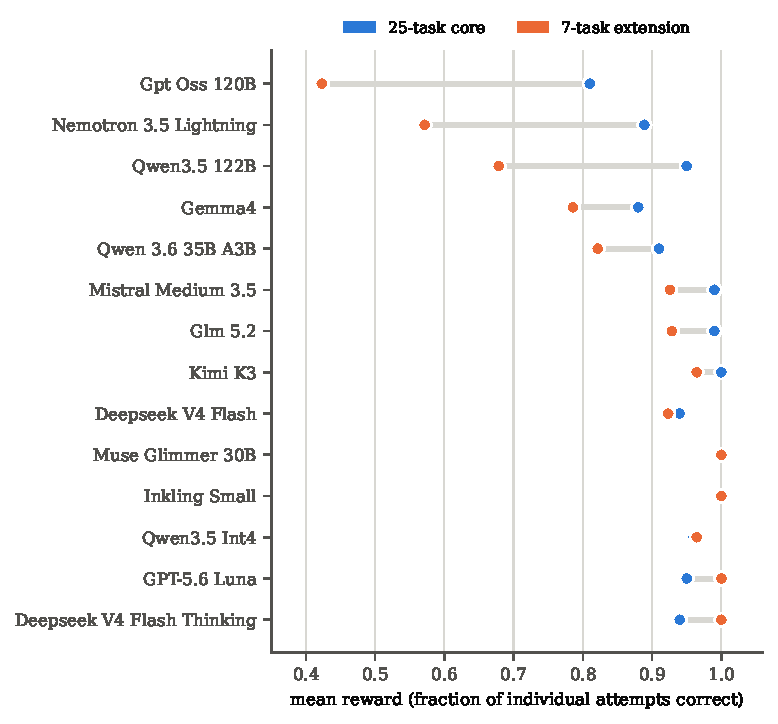
\includegraphics[width=0.76\linewidth]{figures/fig_paired_scopes.pdf}
\caption{Every model evaluated on both parts of the suite. Each row is one model: blue is mean reward on the 25-task core, orange on the extension, and the grey bar is the drop. Models the core cannot separate---several sit at or near 1.000---fan out on the extension.}
\label{fig:paired}
\end{figure}

\begin{table}[t]
\centering
\small
\caption{Models with an included job in \emph{both} scopes on the same provider. Comparing scopes across cohorts would confound task difficulty with model set and serving stack, so only these within-model pairs are admissible. Generated by \texttt{scripts/paired\_scope\_table.py}.}
\label{tab:paired}
\begin{tabular}{llrrrrrr}
\toprule
& & \multicolumn{2}{c}{mean reward} & \multicolumn{2}{c}{pass@1} & \multicolumn{2}{c}{pass@4} \\
\cmidrule(lr){3-4}\cmidrule(lr){5-6}\cmidrule(lr){7-8}
Provider & Model & core & hard & core & hard & core & hard \\
\midrule
e-INFRA & Deepseek V4 Flash & 0.939 & 0.923 & 0.880 & 0.857 & 1.000 & 1.000 \\
e-INFRA & Deepseek V4 Flash Thinking & 0.940 & 1.000 & 0.960 & 1.000 & 1.000 & 1.000 \\
e-INFRA & Gemma4 & 0.880 & 0.786 & 0.880 & 0.714 & 0.920 & 1.000 \\
e-INFRA & Glm 5.2 & 0.990 & 0.929 & 0.960 & 0.857 & 1.000 & 1.000 \\
e-INFRA & Gpt Oss 120B & 0.810 & 0.423 & 0.800 & 0.500 & 0.960 & 0.571 \\
e-INFRA & Kimi K3 & 1.000 & 0.964 & 1.000 & 0.857 & 1.000 & 1.000 \\
e-INFRA & Mistral Medium 3.5 & 0.990 & 0.926 & 1.000 & 0.857 & 1.000 & 1.000 \\
e-INFRA & Qwen3.5 122B & 0.950 & 0.679 & 0.920 & 0.714 & 1.000 & 0.857 \\
e-INFRA & Qwen3.5 Int4 & 0.960 & 0.964 & 0.960 & 0.857 & 1.000 & 1.000 \\
OpenRouter & GPT-5.6 Luna & 0.950 & 1.000 & 0.960 & 1.000 & 1.000 & 1.000 \\
OpenRouter & Inkling Small & 1.000 & 1.000 & 1.000 & 1.000 & 1.000 & 1.000 \\
OpenRouter & Muse Glimmer 30B & 1.000 & 1.000 & 1.000 & 1.000 & 1.000 & 1.000 \\
OpenRouter & Nemotron 3.5 Lightning & 0.889 & 0.571 & 0.917 & 0.571 & 1.000 & 1.000 \\
OpenRouter & Qwen 3.6 35B A3B & 0.910 & 0.821 & 0.960 & 0.857 & 0.960 & 1.000 \\
\bottomrule
\end{tabular}

\end{table}

\paragraph{An outage, and what it cost.}
Hosted evaluation is partly a systems benchmark.
On its first attempt \texttt{kimi-k3} returned \texttt{InternalServerError} from the provider's inference proxy on 24 of its 32 trials, which the error-rate rule correctly excluded; a direct probe of the endpoint returned HTTP 500 on all four requests while the provider's public status page reported the model as online.
Ten hours later the same probe succeeded and a re-run completed 32 of 32 trials with no errors.
We keep both receipts: the failed run is an operational outcome, and the score comes from the clean re-run.
A single evaluation window can misrepresent a model entirely, which is why error accounting belongs in the protocol rather than in a footnote.

\paragraph{Open weights and low price are independent properties.}
Because the OpenRouter provider bills per token, the extension sweep also prices each model, and the spread is larger than the capability spread (Figure~\ref{fig:cost}).
The cheapest run in the cohort is also tied for the best score, while the most expensive model costs roughly thirteen times more for an identical result.
Price follows parameter count, serving efficiency, and provider margin, none of which follow from the licence.
Openness buys the ability to run the weights inside your own boundary---a different and often more valuable property than a low per-token price, and the one that matters for the federated deployment this benchmark is designed around.

\begin{figure}[tbp]
\centering
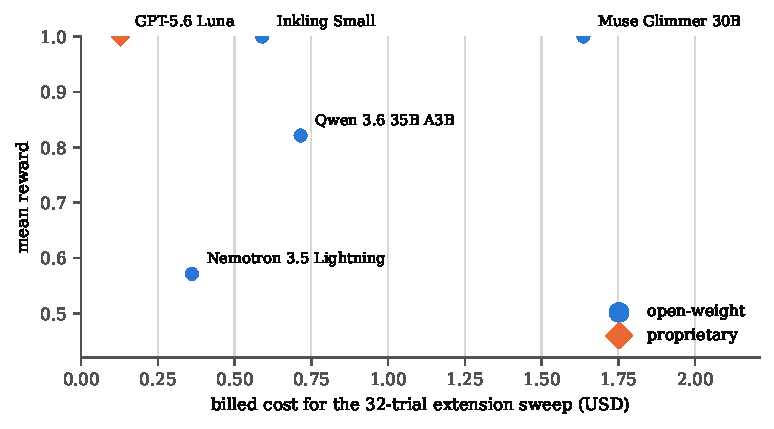
\includegraphics[width=0.72\linewidth]{figures/fig_cost_capability.pdf}
\caption{Billed cost against capability on the extension, OpenRouter cohort. The cheapest run is also tied for the best score, so price is a poor proxy for capability. Weight availability is declared in \texttt{configs/model\_licences.tsv}.}
\label{fig:cost}
\end{figure}

\section{How agents fail}
\label{sec:failures}

A binary verifier records \emph{that} a run failed, not \emph{how}, yet the two are not equally costly.
Because every grader emits an explicit reason before returning zero, the distinction is measurable rather than anecdotal.
We classified all 319 scored failures in the included core cohort from those reasons (Figure~\ref{fig:failures}).

Failures divide into three kinds.
In 68 cases (21.3\%) the agent produced no output file at all---it crashed, ran out of time, or wrote to the wrong path.
In 112 cases (35.1\%) it produced a file that violated the declared structure: 38 had a wrong or missing header, 37 were unparseable JSON, 21 had the wrong number of columns, and 11 put a non-numeric value in a numeric field.
The remaining 139 cases (43.6\%) are the ones that matter most: the file parsed cleanly, satisfied every structural check, and disagreed with the correct answer.
Within these, 97 were wrong numeric or string values in otherwise valid rows and 10 returned the wrong \emph{set} of records---for example an empty BLAST hit list where five hits were expected.

The practical asymmetry is sharp.
The first two kinds announce themselves: a downstream tool refuses to read a missing or malformed file, and the analyst notices immediately.
The third kind does not.
A BED file with correct syntax and wrong coordinates, or a flagstat summary with plausible but incorrect counts, propagates silently into whatever consumes it.
That this quiet mode is the single largest category---and larger than the two loud ones taken separately---is the most important practical result in this paper.

It is also not confined to exotic tasks.
The ten tasks contributing the most failures are ordinary operations: extracting the longest ORF, summarising FASTQ quality, checking trio Mendelian consistency, taking the best BLAST hit, converting GTF to BED.
Header and column-count errors cluster where the output contract specifies an exact schema, which suggests that a meaningful share of failures is specification compliance rather than biology.
That is encouraging for tooling---stricter output validation inside the agent loop would catch much of the loud 56\%---but it does nothing for the quiet 44\%, where only recomputing the answer reveals the error.

\begin{figure}[tbp]
\centering
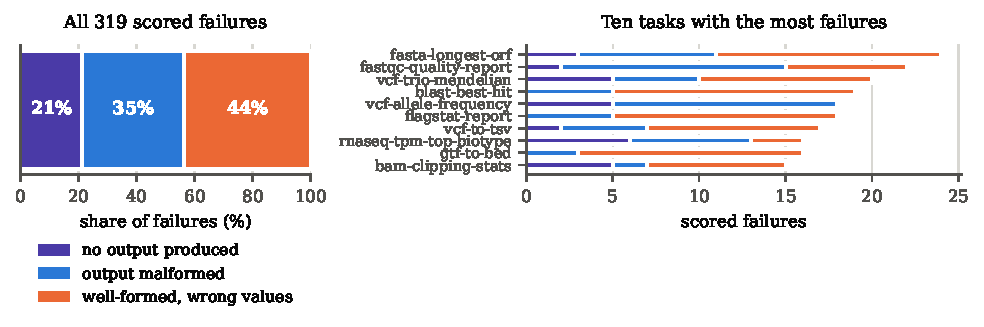
\includegraphics[width=0.96\linewidth]{figures/fig_failure_modes.pdf}
\caption{How runs fail. Left: all 319 scored failures in the included core cohort. Right: the ten tasks contributing the most failures, split the same way. Structurally valid output containing wrong values is the largest single category and is spread across ordinary tasks rather than concentrated in unusual ones.}
\label{fig:failures}
\end{figure}

\subsection*{Which tasks are good measurements?}
\label{sec:irt}

Retiring one item on an item--total correlation invites the obvious follow-up: what do the other items look like under the same lens?
We fitted a two-parameter logistic item response model to every scored trial, treating each task as a test item,
\[
P(\text{correct} \mid \text{model } m, \text{task } t) = \sigma\!\left(a_t (\theta_m - b_t)\right),
\]
with model ability $\theta_m$, task difficulty $b_t$ on the same scale, and discrimination $a_t$.
The fit covers 14 models and 32 tasks; item parameters are each informed by every model's attempts, while ability estimates from fourteen respondents are correspondingly noisy and are reported only as an ordering.

Three results follow, and none of them is comfortable for the benchmark.

\begin{table}[tbp]
\centering
\small
\caption{Item parameters for the ten most difficult tasks, from a 2PL fit over 14 models and 32 tasks. Difficulty is on the ability scale, so a negative value means the task sits below the average model. Discrimination is how sharply the item separates models around that point.}
\label{tab:irt}
\begin{tabular}{lrrr}
\toprule
Task & Pass rate & Difficulty & Discrimination \\
\midrule
\texttt{blast-best-hit} & 0.75 & -0.79 & 3.88 \\
\texttt{vcf-multisample-qc} & 0.79 & -0.85 & 5.06 \\
\texttt{vcf-trio-compound-het} & 0.80 & -0.86 & 7.93 \\
\texttt{rnaseq-featurecounts-matrix} & 0.84 & -0.92 & 6.00 \\
\texttt{vcf-trio-mendelian} & 0.95 & -1.25 & 13.65 \\
\texttt{vcf-diploid-consensus} & 0.78 & -1.28 & 1.24 \\
\texttt{gtf-to-bed} & 0.89 & -1.32 & 2.85 \\
\texttt{bam-depth-histogram} & 0.95 & -1.35 & 5.30 \\
\texttt{fastqc-quality-report} & 0.93 & -1.38 & 3.70 \\
\texttt{fasta-longest-orf} & 0.79 & -1.40 & 1.17 \\
\midrule
\multicolumn{4}{l}{\emph{9 tasks solved on every scored attempt -- no measurement information}} \\
\bottomrule
\end{tabular}

\end{table}

First, \emph{every} task has negative difficulty on the fitted ability scale, the hardest---\texttt{blast-best-hit} at $-0.79$---still sitting well below the average model.
This is the saturation result stated psychometrically rather than as a pass rate: the suite as a whole is calibrated below the population it is being used to measure.

Second, nine of the 32 tasks were solved on every scored attempt by every model.
Their difficulty and discrimination are set by the prior rather than by data, because a task nobody fails carries no information about who is stronger.
They remain useful as regression tests---a future model that fails \texttt{tpm-normalize} has broken something basic---but they contribute nothing to ranking and should not be counted as evidence that a model is capable.

Third, discrimination varies more than difficulty does, and the two are not aligned.
\texttt{vcf-trio-mendelian} discriminates sharply ($a = 13.7$) despite a 0.95 pass rate, because the models that fail it are exactly the weaker ones.
Meanwhile four tasks discriminate weakly at $a < 1$ despite non-trivial failure rates: \texttt{rnaseq-tpm-top-biotype}, \texttt{fasta-6frame-codon-counts}, \texttt{vcf-to-tsv}, and \texttt{kmer-contamination-mixture}.
Failures on these are closer to noise than to signal---a strong model fails them about as often as a weak one---which makes them the next candidates for revision, and notably one of them is a member of the harder extension.
Selecting future tasks on discrimination rather than on pass rate is the concrete methodological lesson: a task in the 10--80\% band can still be a poor item, and our original selection rule could not tell the difference.

\section{Discussion}

\subsection*{What hardware do you actually need?}
\label{sec:deployment}

For a laboratory the practical question is not which model scores highest but which model it can run at all, and the two answers are further apart than one might expect.
Table~\ref{tab:hardware} places every model in the e-INFRA panel on a hardware ladder, using weight memory at the served precision---total parameters multiplied by bytes per parameter---as the sizing quantity.
This is a floor rather than a deployment specification: the key--value cache for a 256K--1M context, activations, and runtime buffers add substantially on top, and a mixture-of-experts model needs its \emph{whole} weight set resident even though only the active parameters run per token.
As a sanity check on the arithmetic, the released MXFP4 weights of Kimi~K3 are reported at roughly 1.4~TB, which is what 2.8T parameters at half a byte each predicts, and its vendor recommends 64 or more accelerators.

\begin{table}[tbp]
\centering
\small
\caption{What it takes to self-host each model in the e-INFRA panel. Weight memory is total parameters at the served precision and excludes KV cache and runtime overhead. Tier A models are within reach of a workstation once quantised to four bits; tier E needs a multi-node cluster.}
\label{tab:hardware}
\begin{tabular}{llrrl}
\toprule
Model & Total (active) & Precision & Weights (GB) & Hardware needed \\
\midrule
GPT-OSS-120B & 120B (A5.1B) & \texttt{mxfp4} & 60 & B: one datacentre GPU \\
Gemma 4 & 31B (31B) & \texttt{bf16} & 62 & A: laptop or workstation \\
Qwen3.5 122B & 122B (A10B) & \texttt{fp8} & 122 & B: one datacentre GPU \\
Mistral Medium 3.5 & 128B (128B) & \texttt{fp8} & 128 & B: one datacentre GPU \\
Qwen3.5 Int4 & 397B (A17B) & \texttt{int4} & 198 & C: 2--4 GPU server \\
DeepSeek V4 Flash & 304B (A13B) & \texttt{fp8} & 304 & C: 2--4 GPU server \\
DeepSeek V4 Flash Thinking & 304B (A13B) & \texttt{fp8} & 304 & C: 2--4 GPU server \\
GLM 5.2 & 756B & \texttt{fp8} & 756 & D: full 8-GPU node \\
Kimi K3 & 2.8T (A104B) & \texttt{fp8} & 2800 & E: multi-node cluster \\
\bottomrule
\end{tabular}

\end{table}

The ladder spans two orders of magnitude, from a 31B dense model that fits a laptop after 4-bit quantisation to a 2.8T mixture-of-experts model that fits no single machine.
Capability follows it weakly and with a ceiling: across the eight scored models the rank correlation between weight memory and mean reward is $\rho = 0.77$ ($p = 0.027$), but the relationship saturates---the four models at or above 130~GB score 0.800--0.875, so a move from a two-GPU server to an eight-GPU node buys nothing measurable---and admits large inversions, with 62~GB Gemma~4 outscoring 122~GB Qwen3.5~122B.
Recency does not explain it either ($\rho = 0.53$, $p = 0.18$), and size and release date are themselves confounded in this panel ($\rho = 0.76$), so at $n = 8$ neither can substitute for running the benchmark on the model one intends to deploy.

\begin{figure}[tbp]
\centering
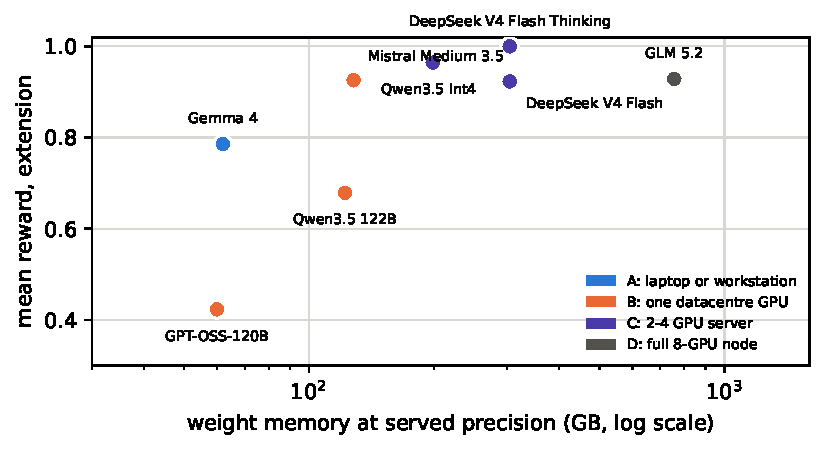
\includegraphics[width=0.76\linewidth]{figures/fig_hardware_vs_score.pdf}
\caption{Capability against the hardware needed to host it. Colour marks the tier from Table~\ref{tab:hardware}. Larger models score better on average ($\rho = 0.77$, $p = 0.027$), but the relationship saturates above roughly 130~GB and admits large inversions: the 62~GB workstation-class model outscores a 122~GB model that needs a datacentre GPU.}
\label{fig:hardware}
\end{figure}

Three deployment routes follow from this, and they map onto real institutional constraints.
A laboratory with no privacy constraint and no GPU budget should use a commercial aggregator: the entire 8-task sweep cost between \$0.15 and \$1.94 per model, which is less than the electricity of running it locally, at the cost of sending prompts and data to third-party infrastructure.
A laboratory working with controlled-access data and access to institutional hardware---the arrangement e-INFRA CZ provides for ELIXIR CZ members---can host a tier B or C model inside the administrative boundary and reach the top of the observed score range.
A laboratory that must keep data on a single machine is restricted to tier A, and the encouraging finding is that this is no longer a severe restriction: a workstation-class model already solves the great majority of the 25-task core and roughly two thirds of the extension.

We did not measure tier A execution directly, and that is the main gap in this analysis.
Our fixtures are deliberately sized for it, but confirming which models remain usable at 4-bit on consumer hardware---and how much quantisation costs in reliability rather than in benchmark score---requires its own study.

\subsection*{What to delegate today}

The per-task results support a more specific recommendation than a single score.
Format conversion and summarisation---GTF to BED, VCF to TSV, FASTA statistics, flagstat-style counting---are solved reliably by every model at the top of both cohorts, and are reasonable to delegate with spot-checking.
Multi-stage reasoning over biological structure is not: joining CIGAR-derived splice junctions to annotations was solved by 2 of 13 models, and trio-aware and diploid-consensus variant logic separates models sharply.
Between these lie tasks that are solved but not dependably, where the model produces a correct answer most of the time and a plausible wrong one otherwise; these are exactly the cases where an unchecked result is most costly, and where a second run and a comparison is cheap insurance.

The general rule this suggests is that delegation is safe in proportion to how mechanically checkable the output is.
An agent that writes a BED file can be checked by re-deriving a handful of rows; an agent that produces a filtered variant set with a subtle inheritance error cannot be checked without redoing the analysis.

\subsection*{Limitations and reproducibility}

One operational deviation is recorded for completeness: a single core-25 job (\texttt{deepseek-v4-flash}) ran at four concurrent trials rather than two, because a ceiling change was applied to an already-running orchestrator that had loaded the previous value.
Concurrency affects queueing and wall-clock, not task content or grading, so the job's scores are retained; its wall-clock is not comparable with the rest of the cohort, which is in any case not reported as a model-speed measurement.

This draft stops short of claiming final e-INFRA results that have not yet been run: the harder-task subset is frozen, but the e-INFRA cohort remains an extension in progress, so the quantitative claims here are limited to artefacts stored in the repository as of August 12, 2026.

Four limitations bound the analysis.
The main table uses only the clean repeated OpenRouter cohort rather than the older $k=1$ and $k=3$ sweeps; 25 core tasks make every interval wide; cost and wall-clock are not comparable across shared hosted services; and holding the scaffold fixed at Terminus-2 controls a large variance source while bounding external validity, since a different scaffold can move scores substantially for the same model.

A binary verifier records that a task failed without recording how it failed, and the two failure families have very different practical costs.
An absent or malformed artifact is cheap, because it announces itself: a downstream tool refuses to read it.
A well-formed but incorrect artifact is expensive, because nothing flags it and the error propagates into whatever consumes it.
Because our graders emit an explicit reason before returning zero, this split is measurable rather than speculative.
Classifying all 319 scored failures in the included cohort by the verifier's own reason gives 68 (21.3\%) missing outputs, 112 (35.1\%) structurally invalid outputs---wrong header, wrong column count, unparseable JSON, non-numeric fields---and 139 (43.6\%) outputs that parsed cleanly and disagreed with the gold answer.
The quiet failure mode is thus the single largest category, and it is spread across ordinary tasks rather than concentrated in exotic ones: \texttt{blast-best-hit}, \texttt{fasta-longest-orf}, \texttt{flagstat-report}, \texttt{gtf-longest-transcript-cds}, and \texttt{gtf-to-bed} each contribute 13--14 such failures.
For a reader weighing unsupervised delegation this is the most important number in the paper: when these models fail, the most common single outcome is a plausible file containing wrong numbers.
The classifier is released as \texttt{scripts/summarize\_failure\_modes.py} with its per-trial output, so the taxonomy can be recomputed on any future cohort.

Reproducibility is built in: the repository contains the summarizer, the generated CSV and \LaTeX{} tables, and explicit exclusion logic, so every number and figure here regenerates from raw receipts with one command.
The three task images pin every bioinformatics dependency to an explicit version---\texttt{samtools} and \texttt{bcftools} 1.21, \texttt{minimap2} 2.28, \texttt{bedtools} 2.31.1---though they are published by tag rather than immutable digest, which is worth hardening before archival.

\paragraph{Availability.}
Tasks, images, runners, graders, the analysis scripts used for every table in this paper, and the frozen selection receipt are available at \url{https://github.com/ML-Bioinfo-CEITEC/BioTerm-Bench}.
Raw Harbor job directories are large and are retained locally; the derived per-model, per-task, and per-failure CSVs that back the tables are generated by \texttt{scripts/summarize\_bioterm\_v2.py} and \texttt{scripts/summarize\_failure\_modes.py}.
This draft therefore provides a concrete baseline for the next iteration: land the harder tasks, run the e-INFRA cohort under the same repeated protocol, and keep protocol failures visible as first-class experimental outcomes rather than burying them in summary averages.

\subsection*{Future directions}

Three extensions would sharpen what this benchmark can say.

The first is to close the deployment gap.
We evaluated hosted inference on a commercial aggregator and on institutional hardware, but not the strictest case: weights executed on the analyst's own machine through a local runtime such as Ollama \citep{ollama} or LM~Studio.
Our fixtures are sized for it, and the tier~A result---a workstation-class model already solving most of the core---suggests the answer would be encouraging, but quantisation to four bits may cost reliability in ways a benchmark score hides.

The second is to look backwards rather than forwards.
Every model here was released within roughly a year, which is why size and recency could not be separated.
Evaluating models from the preceding two years---many no longer served by either provider, but still available as weights---would turn a snapshot into a trajectory and show how quickly routine bioinformatics became automatable.

The third is to keep the suite ahead of the field.
Nine of 32 tasks are already solved on every attempt by every model, and retiring the one genuinely hard extension task left the remainder saturated at the top.
The next pack should be selected on discrimination rather than pass rate, and should deliberately include tasks that current frontier models fail.

\section{Conclusion}

BioTerm-Bench is close to the point where its original 25-task core is no longer sufficient as the primary discriminator among current small open models.
The existing OpenRouter artefacts already show partial saturation in mean reward, continued benefit from repeated attempts, and enough provider-path instability that operational filtering must be part of the benchmark protocol.
The core keeps its value as a continuity score and as evidence of what is now routinely automatable, while the harder pack carries the discriminative load until it too saturates.

For a practitioner weighing whether an agent can absorb routine terminal work, the evidence here supports a narrow conclusion rather than a comfortable one.
On tightly specified single-artifact tasks the strongest small open models are usually right, and repeated attempts recover much of what a single attempt misses.
But the recovery requires someone who can tell a right answer from a wrong one, and the most common single failure mode is a well-formed file containing wrong numbers.
The realistic role today is therefore an accelerator for someone who could have done the task themselves, not a replacement for that person.

\section*{Data availability}

The task suite, container definitions, graders, runners, and analysis scripts are available at \url{https://github.com/ML-Bioinfo-CEITEC/BioTerm-Bench} under the Apache~2.0 licence.
The derived per-model, per-task, and per-failure tables that back every figure and table in this paper are regenerated from raw run receipts by \texttt{scripts/refresh\_paper\_tables.sh}.
Raw Harbor job directories are large and are retained by the authors; they are available on request.

\section*{Conflict of interest}

The authors declare no competing financial or non-financial interests.

\section*{Acknowledgements}

This work was supported by [FUNDING BODY] under grant [GRANT NUMBER]. % template -- complete before submission
Computational resources were provided by the e-INFRA CZ project (ID:90254), supported by the Ministry of Education, Youth and Sports of the Czech Republic.

{\small
\setlength{\bibsep}{2pt}
\bibliographystyle{plainnat}
\bibliography{references}
}

\appendix

\section{Hard-subset selection receipt}
\label{app:selection}

Table~\ref{tab:v2-selection} reproduces the frozen per-task development record that fixed the retained eight tasks before any evaluation model was run.
It is included so the selection can be audited against the evaluation outcome in Section~\ref{sec:results} without re-deriving it from the repository.

\begin{table}[h]
\centering
\small
\caption{Frozen retained hard-subset tasks from \texttt{notes/v2\_task\_selection.json}. Rates use only scored development attempts; errors are preserved separately and do not enter the rate denominator.}
\label{tab:v2-selection}
\begin{tabular}{llrrr}
\toprule
Task & Category & Passes / scored & Errors & Rate \\
\midrule
\texttt{bam-splice-junction-support} & alignment & 1 / 4 & 2 & 0.25 \\
\texttt{vcf-diploid-consensus} & variant & 1 / 6 & 0 & 0.17 \\
\texttt{vcf-trio-compound-het} & variant & 1 / 5 & 1 & 0.20 \\
\texttt{vcf-multisample-qc} & qc & 2 / 5 & 1 & 0.40 \\
\texttt{rnaseq-featurecounts-matrix} & rnaseq & 2 / 6 & 0 & 0.33 \\
\texttt{rnaseq-deseq2-contrast} & rnaseq & 2 / 5 & 1 & 0.40 \\
\texttt{kmer-contamination-mixture} & qc & 2 / 6 & 0 & 0.33 \\
\texttt{ortholog-rbh-clusters} & search & 4 / 6 & 0 & 0.67 \\
\bottomrule
\end{tabular}

\end{table}

\section{A worked example}
\label{app:example}

At the atomic end of the ladder, \texttt{gtf-to-bed} gives the agent a 21\,KB GTF file of chromosome~22 gene annotations inside a container carrying the usual HTS stack, and an instruction that fixes the output contract exactly: write \texttt{/app/output/exons.bed} as a BED6 TSV with one row per \texttt{exon} record, \texttt{start} converted to 0-based half-open coordinates, \texttt{name} taken from the \texttt{gene\_id} attribute with quotes stripped, a literal \texttt{.} in the score column, rows sorted by chromosome, start, end, and name, and duplicate rows preserved rather than collapsed.
The grader rejects any row that does not carry exactly six tab-separated columns and then compares the produced file against a stored gold file after normalization; the reward is 1 on an exact match and 0 otherwise.
No model judges any output.
Tasks at the hard end of the ladder keep the same contract discipline but require several coupled stages, such as joining CIGAR-derived splice junctions to GTF annotations.

\section{Audit tables for the core-25 cohort}
\label{app:audit}

These two tables are retained for auditing rather than for the argument in the main text: Table~\ref{tab:exclusions} records which jobs the error-rate rule removed and why, and Table~\ref{tab:hardest} records residual task-level difficulty in the current core.

\begin{table}[h]
\centering
\small
\caption{Excluded OpenRouter jobs. These are not counted as scientific failures because the trial artefacts do not support normal benchmark interpretation under the error-rate policy.}
\label{tab:exclusions}
\begin{tabular}{llrrr}
\toprule
Model & Reason & Error rate & Error trials & Verifier cov. \\
\midrule
GLM 4.5 Air & protocol failure high error rate & 1.00 & 100 & 0.00 \\
Ministral 14B & protocol failure high error rate & 1.00 & 100 & 0.00 \\
Ministral 8B & protocol failure high error rate & 1.00 & 100 & 0.00 \\
Mistral Nemo & protocol failure high error rate & 1.00 & 100 & 0.00 \\
Mistral Small 2501 & protocol failure high error rate & 0.60 & 60 & 0.49 \\
Mistral Small 2603 & protocol failure high error rate & 1.00 & 100 & 0.00 \\
Mistral Small 3.1 24B & protocol failure high error rate & 1.00 & 100 & 1.00 \\
Qwen 2.5 7B & protocol failure high error rate & 0.97 & 97 & 0.11 \\
Qwen 3.6 Flash & protocol failure high error rate & 1.00 & 100 & 0.00 \\
Ministral 3B 2512 & unfinished & 0.02 & 2 & 0.03 \\
\bottomrule
\end{tabular}

\end{table}

\begin{table}[h]
\centering
\small
\caption{Hardest tasks in the current clean OpenRouter cohort. ``Disc.'' is an item-discrimination statistic computed against the model-level pass@4 totals on the remaining tasks.}
\label{tab:hardest}
\begin{tabular}{llrrr}
\toprule
Task & Category & pass@4 models & Mean reward & Disc. \\
\midrule
fastqc-quality-report & qc & 3/8 & 0.208 & 0.73 \\
blast-best-hit & search & 3/8 & 0.240 & 0.69 \\
fasta-longest-orf & metadata & 4/8 & 0.250 & 0.91 \\
vcf-trio-mendelian & variant & 4/8 & 0.312 & 0.91 \\
gtf-to-bed & metadata & 4/8 & 0.375 & 0.91 \\
vcf-to-tsv & metadata & 4/8 & 0.417 & 0.62 \\
\bottomrule
\end{tabular}

\end{table}

\end{document}
